\documentclass[12pt, a4paper]{article}
\usepackage[spanish]{babel}
\usepackage[utf8]{inputenc}
\usepackage{graphicx}
\usepackage{geometry}
\usepackage{fancyhdr}
\usepackage{float}
\usepackage{titling}

\geometry{a4paper, margin=2.5cm}
\pagestyle{fancy}
\fancyhf{}
\rhead{
\includegraphics[height=1.2cm]{images/logo-usm.png}} % Logo en encabezado
\lhead{Grupo 19\\Visualización de Datos}
\rfoot{Página \thepage}

% Configuración del logo en portada
\pretitle{
  \begin{center}
  \vspace{1cm}
  
\includegraphics[width=0.5\textwidth]{images/logo-usm.png}\\
  \vspace{1.5cm}
  \LARGE
}
\posttitle{\end{center}}

\title{Informe: Tecnología en la Vida Cotidiana}
\author{Felipe Campaña, Javier Gómez, Matias Elgueta}
\date{\today\\[2cm]
}

\begin{document}

\maketitle

\section*{Criterios de Selección}
\begin{itemize}
    \item Criterio 1: Horas en redes sociales por país
    \item Criterio 2: Evolución de clientes telecomunicación
    \item Criterio 3: **
    \item Criterio 4: **
    \item Criterio 5: **
    \item Criterio 6: **
\end{itemize}

\section*{Análisis Gráfico}

% Repite este bloque para cada gráfico (total 6)
\subsection*{Gráfico 1: Aquí colocar título}
\begin{figure}[H]
    \centering
    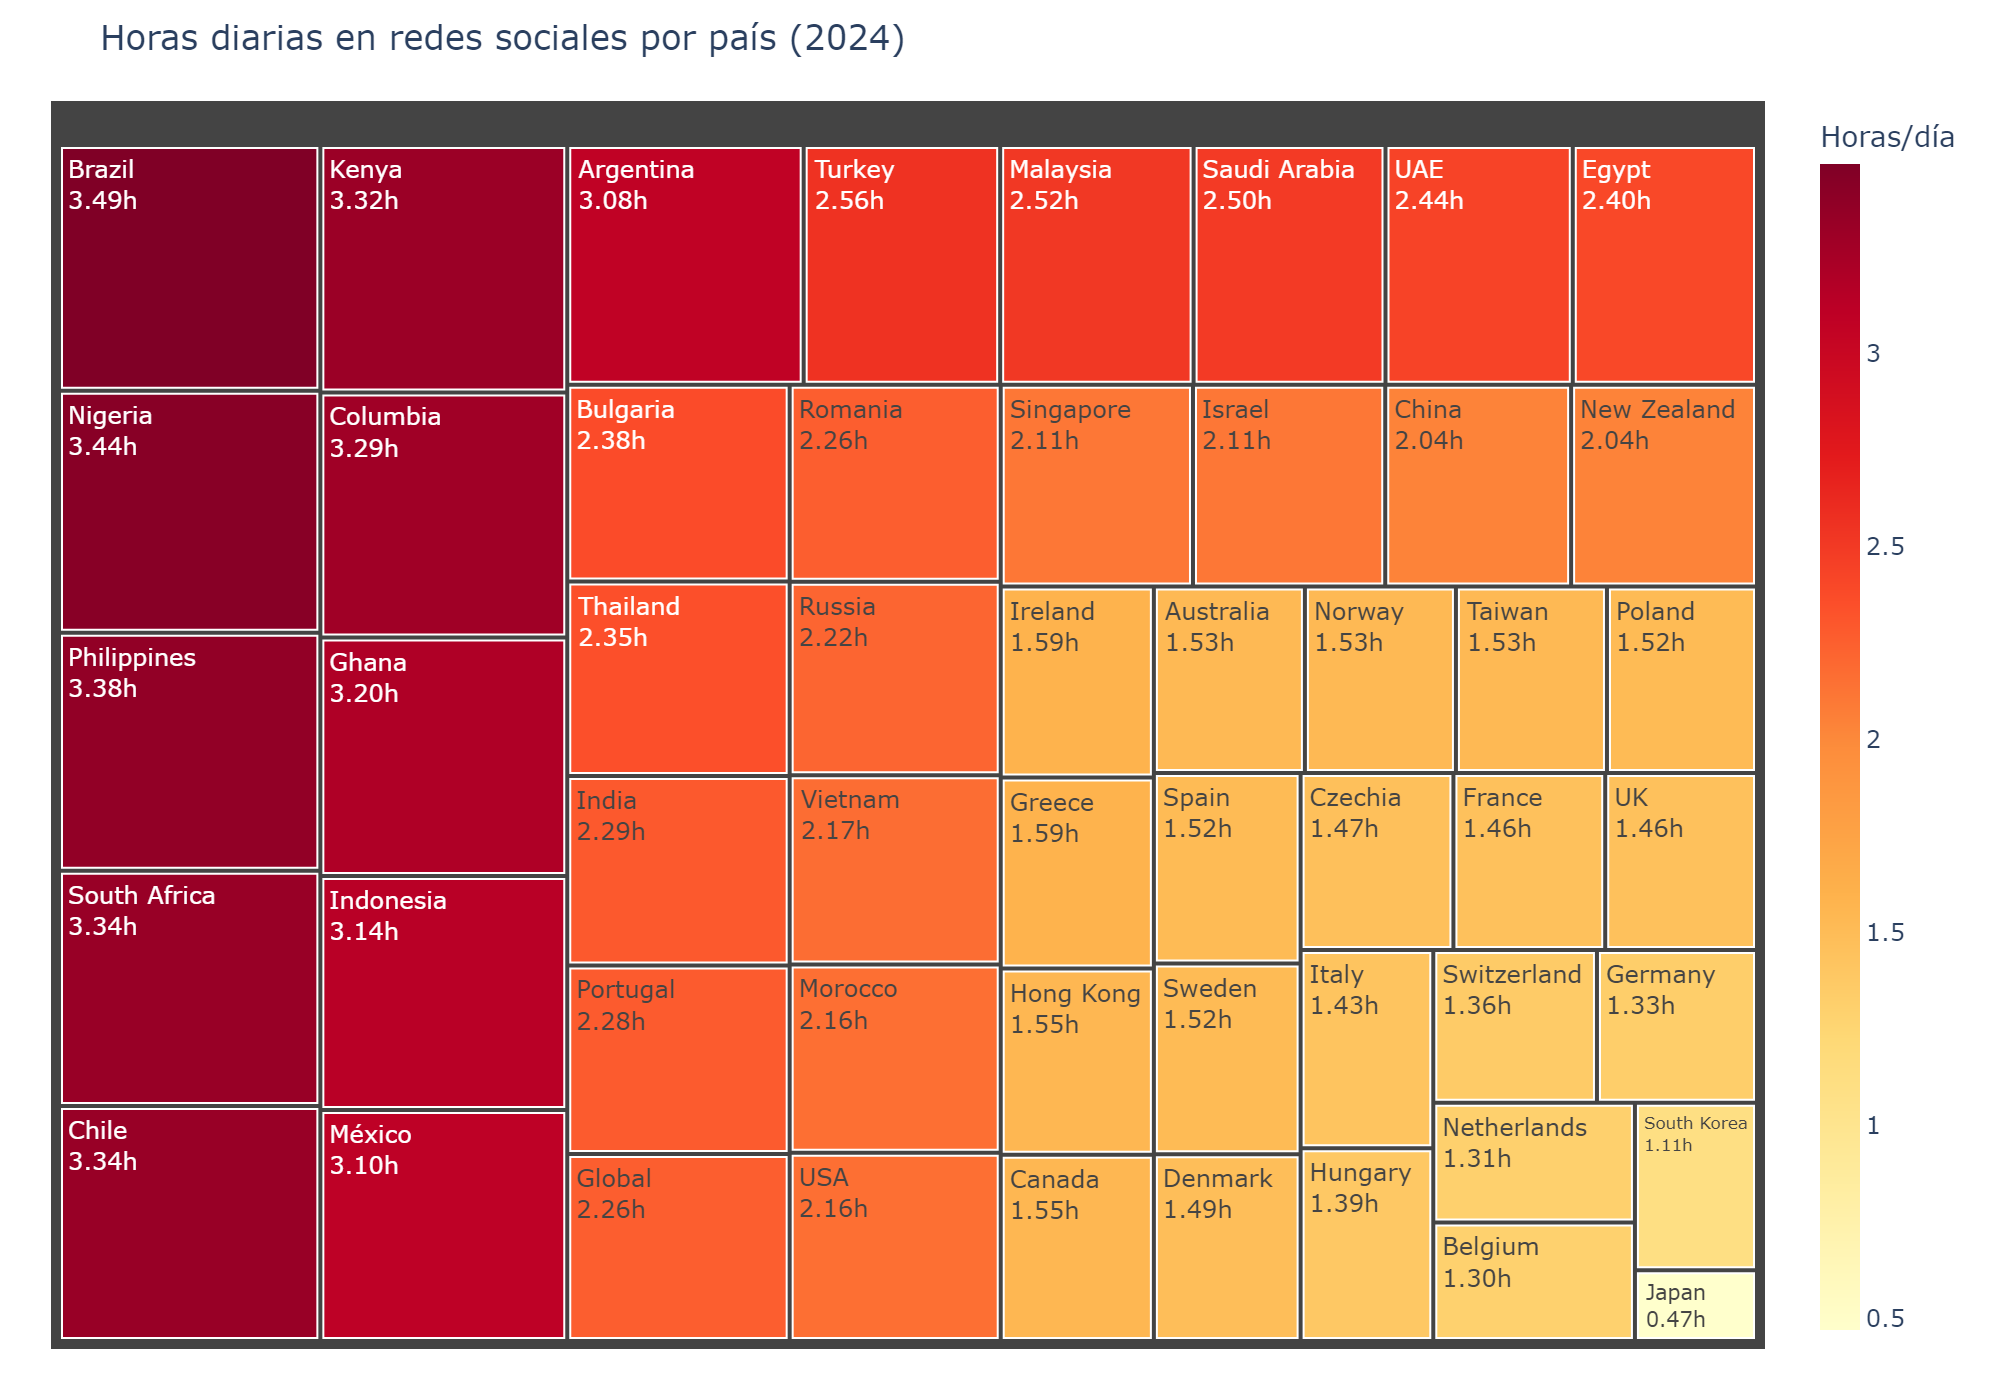
\includegraphics[width=0.85\textwidth]{images/graph1_JG.png}
    \caption{Fuente: Elaboración propia con datos de [Nombre de Fuente]}
\end{figure}

\subsubsection*{Conclusión}
Texto de conclusión específico para este gráfico. Analizar tendencias observadas y su relación con el impacto tecnológico en la vida cotidiana.

% Gráfico 2
\subsection*{Gráfico 2: Aquí colocar título}
\begin{figure}[H]
    \centering
    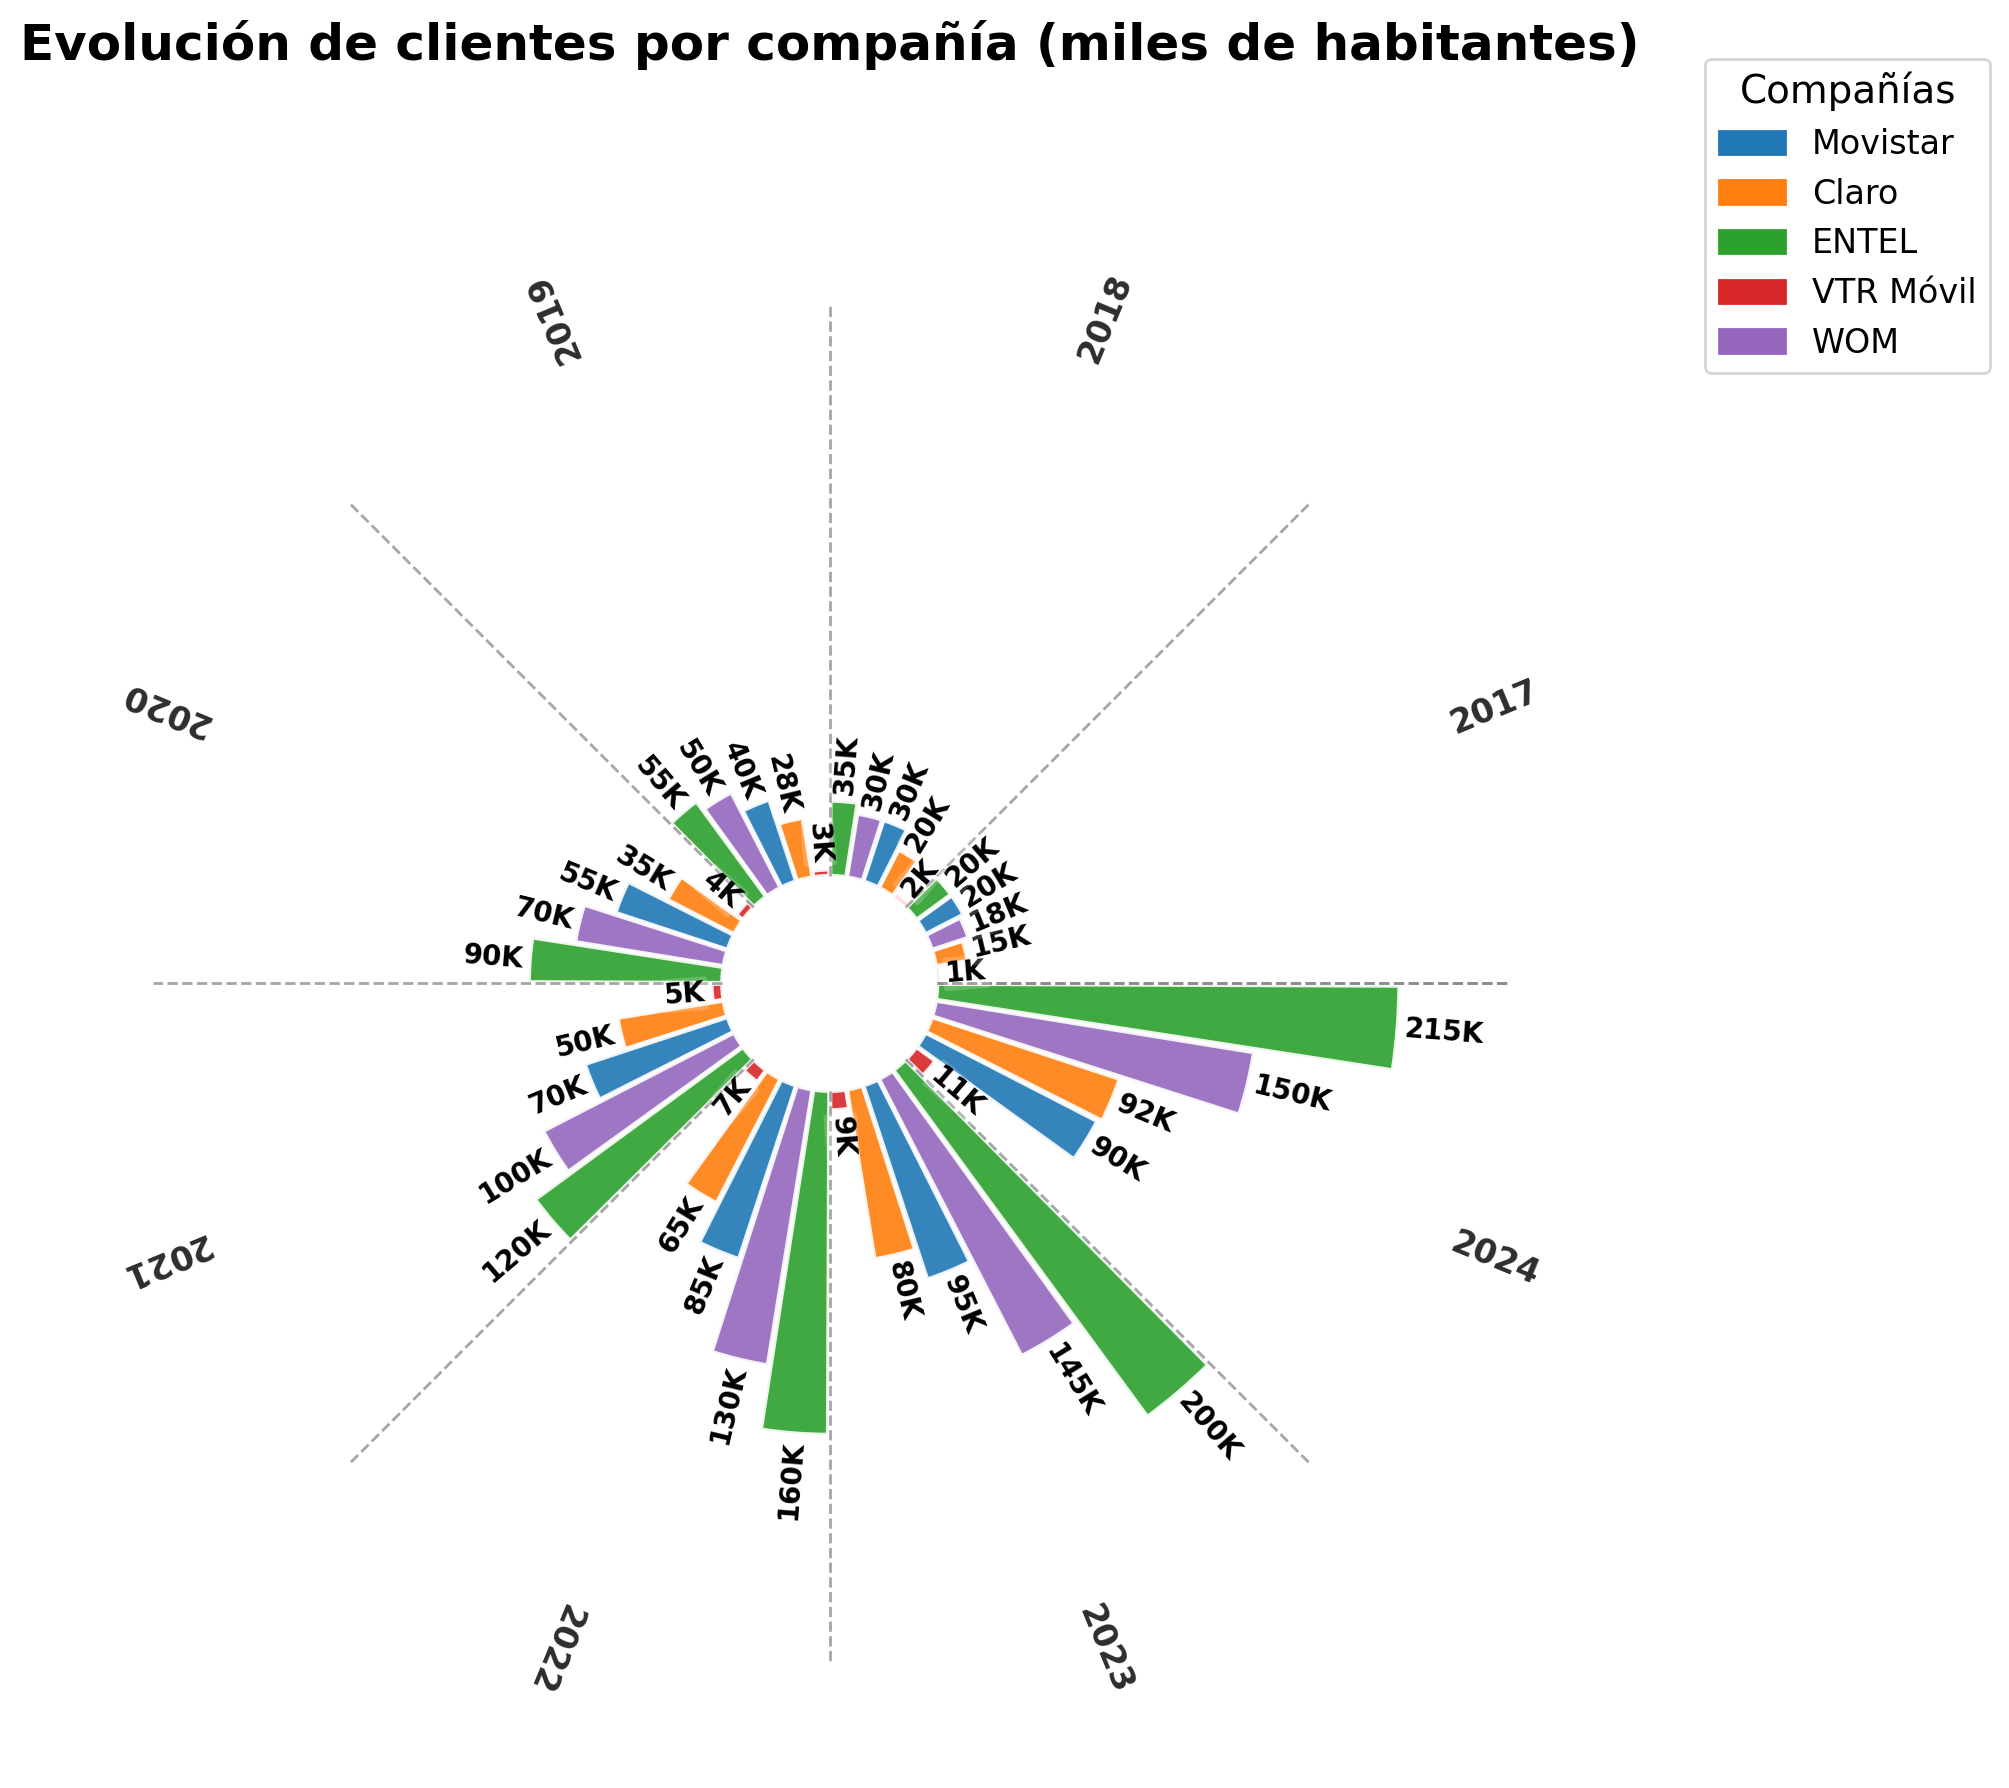
\includegraphics[width=0.85\textwidth]{images/graph2_JG.png}
    \caption{Fuente: Elaboración propia con datos de [Nombre de Fuente]}
\end{figure}

\subsubsection*{Conclusión}
Texto de conclusión específico para este gráfico. Analizar tendencias observadas y su relación con el impacto tecnológico en la vida cotidiana.

% Añadir los gráficos 3 al 6 siguiendo el mismo patrón

\section*{Conclusiones Generales}
\begin{itemize}
    \item Opcional**
  
\end{itemize}

\end{document}
